\documentclass[11pt]{amsart}
\usepackage{geometry}                % See geometry.pdf to learn the layout options. There are lots.
\geometry{letterpaper}                   % ... or a4paper or a5paper or ...
%\geometry{landscape}                % Activate for for rotated page geometry
%\usepackage[parfill]{parskip}    % Activate to begin paragraphs with an empty line rather than an indent
\usepackage{graphicx}
\usepackage{amssymb}
\usepackage{epstopdf}
\usepackage[usenames,dvipsnames]{color}
\usepackage{hyperref}
\usepackage{subfig}
\hypersetup{colorlinks=true}
\DeclareGraphicsRule{.tif}{png}{.png}{`convert #1 `dirname #1`/`basename #1 .tif`.png}
\renewcommand\familydefault{\sfdefault}
\newcommand{\todo}[1]{{\bf\textcolor{red}{TODO: #1}}}
\setlength{\topmargin}{0cm}
\setlength{\headheight}{0cm}
\setlength{\headsep}{1cm}
\setlength{\textheight}{7.7in}
\setlength{\textwidth}{6.5in}
\setlength{\oddsidemargin}{0cm}
\setlength{\evensidemargin}{0cm}
\setlength{\parindent}{0.25cm}
\setlength{\parskip}{0.1cm}

\usepackage{prettyref}
\newrefformat{sec}{Section~\ref{#1}}
\newrefformat{tbl}{Table~\ref{#1}}
\newrefformat{fig}{Figure~\ref{#1}}
\newrefformat{chp}{Chapter~\ref{#1}}
\newrefformat{eqn}{\eqref{#1}}
\newrefformat{set}{\eqref{#1}}
\newrefformat{alg}{Algorithm~\ref{#1}}
\newrefformat{apx}{Appendix~\ref{#1}}
\newcommand\pr[1]{\prettyref{#1}}

\usepackage{fancyhdr,graphicx,lastpage}% http://ctan.org/pkg/{fancyhdr,graphicx,lastpage}
\fancypagestyle{plain}{
  \fancyhf{}% Clear header/footer
  \fancyhead[L]{CSCI-GA.3033-018 - Geometric Modeling}% Right header
  \fancyhead[R]{
\includegraphics[height=20pt]{nyu.pdf}}% Right header
  \fancyfoot[L]{\vspace{2pt} Daniele Panozzo}% Left footer
  \fancyfoot[R]{\vspace{2pt} \thepage}% Right footer
}

\renewcommand{\vec}[1]{\mathbf{#1}}
\DeclareMathOperator*{\argmin}{argmin}
\def\x{\vec{x}}
\def\c{\vec{c}}
\def\p{\vec{p}}
\providecommand{\abs}[1]{\lvert#1\rvert}
\providecommand{\norm}[1]{\lVert#1\rVert}

\begin{document}

\hspace{50pt}

\begin{center}

{\huge \textbf{Assignment 2: Implicit Surface Reconstruction}}\\
\end{center}

In this exercise you will
\begin{itemize}
\item{Compute an implicit MLS function approximating a 3D point cloud with
    given (but possibly unnormalized) normals.}
\item{Sample the implicit function on a 3D volumetric grid.}
\item{Apply the marching cubes algorithm to extract a triangle mesh of this zero
    level set.}
\item{Experiment with various MLS reconstruction parameters.}
\end{itemize}

Your main task is to construct an implicit function $f(\x)$ defined on all
$\x \in \mathbb{R}^3$ whose zero level set contains (or at least passes near)
each input point. That is, for every point $\p_i$ in the point cloud, we want
$f(\p_i) = 0$. Furthermore, $\nabla f$ (the isosurface normal) evaluated at
each point cloud location should approximate the point's normal provided as
input.

You will construct $f$ by interpolating a set of target values, $d_i$, at
``constraint locations,'' $\c_i$. The MLS interpolant is defined by minimization
of the form $f(\x) = \argmin_\phi \sum_{i} w(\c_i, \x) (\phi(\c_i) -
d_i)^2$, where $\phi(\x)$ lies in the space of admissible function (e.g.,
multivariate polynomials up to some degree) and $w$ is a weight function that
prioritizes each constraint equation depending on the evaluation point, $\x$.

\emph{Note:} The datasets provided actually already include triangles.
Ignore them for this assignment.

\section{Setting up the Constraints}
\label{sec:constraints}
Your first step is thus to build the set of constraint equations by choosing
constraint locations and values. Naturally, each point $\vec{p}_i$ in the input
point cloud should contribute a constraint with target value $d_i = 0$. But
these constraints alone provide no information to distinguish the object's
inside (where we want $f < 0$) from its outside (where we want $f > 0$). Even
worse, the minimization is likely to find the trivial solution $f = 0$ (if it
lies in the space of admissible functions). To address these problems, we
introduce additional constraints incorporating information from the normals as
follows:

\begin{itemize}
\item For each point $\vec{p}_i$ in the point cloud, add a constraint of the form $f(\vec{p}_i) = 0$.
\item Fix an $\varepsilon$ value, for instance $\varepsilon = 0.01\times  \textrm{bounding\_box\_diagonal}$.
\item For each point $\vec{p}_i$ compute $\vec{p}_{i+N} = \vec{p}_i +
    \varepsilon \vec{n}_i$, where $\vec{n}_i$ is the normalized normal of
        $\vec{p}_i$. Check that $\vec{p}_i$ is the closest point to $\vec{p}_{i+N}$;
        if not, halve $\varepsilon$ and recompute $\vec{p}_{i+N}$ until
        this is the case. Then, add another constraint equation:
        $f (\vec{p}_{i+N} ) = \varepsilon$.
\item Repeat the same process for $-\epsilon$, i.e., add equations of the form
    $f(\vec{p}_{i+2N}) = -\epsilon$. Do not forget to check each time that $\vec{p}_i$ is the closest point to $\vec{p}_{i+2N}$ .
\end{itemize}
After these steps, you should have $3n$ equations for the implicit function
$f(\x)$.

\begin{figure}[h!]
   \centering
   \subfloat[Input point cloud]{\label{fig:cat_blackpts}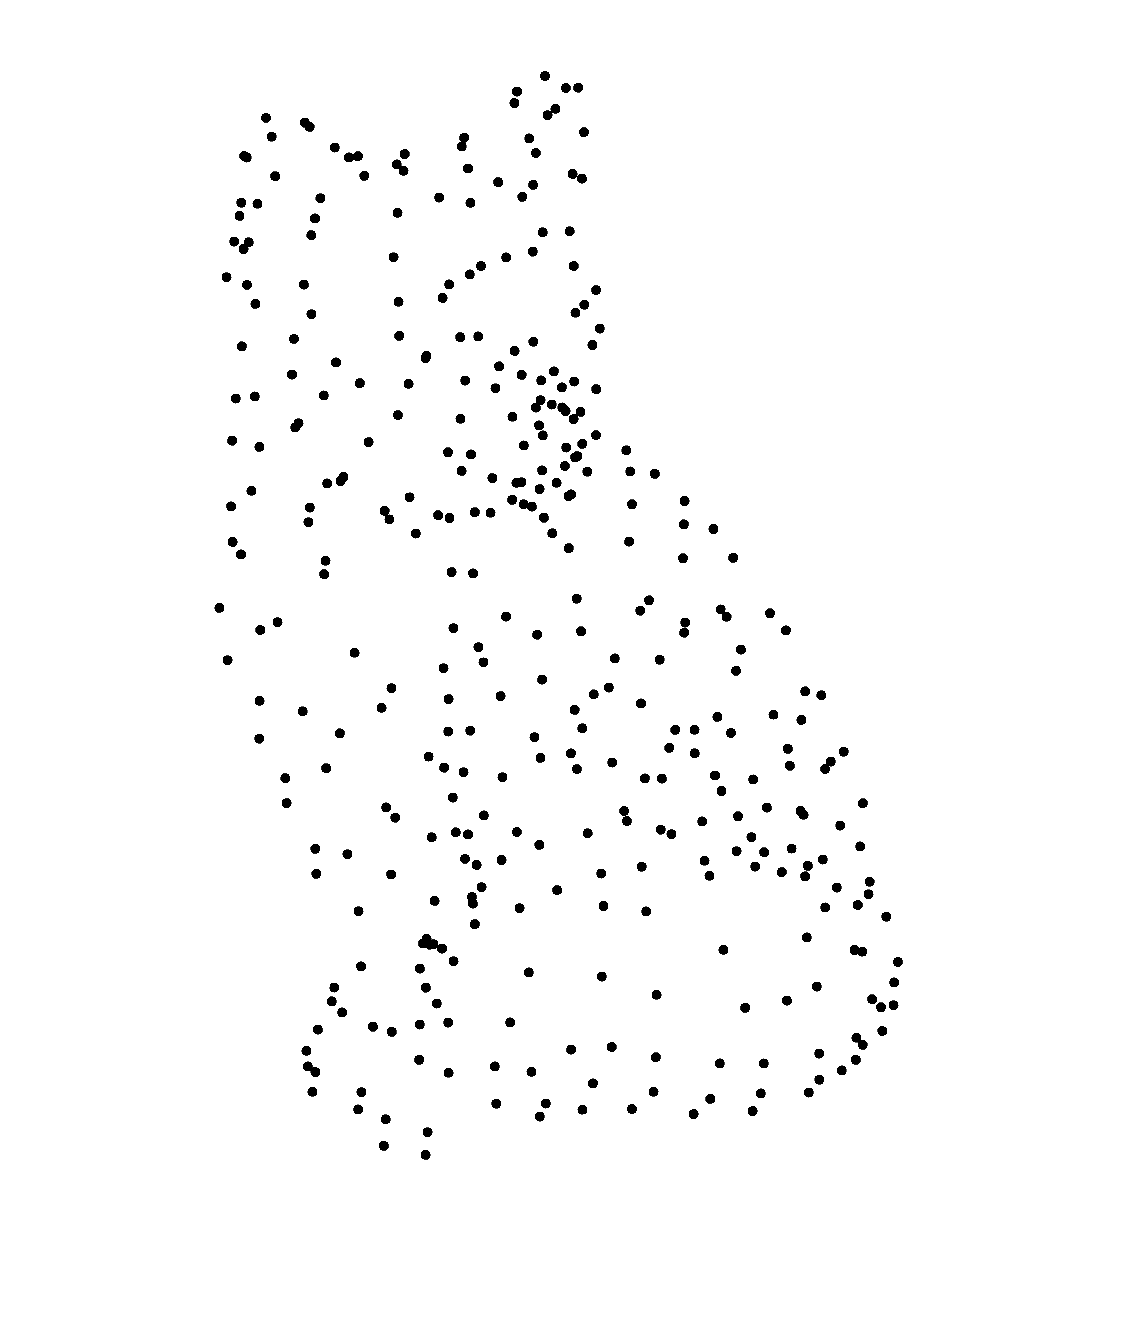
\includegraphics[width=0.4\linewidth]{cat_blackpts.png}} % requires the graphicx package
\hspace{1cm}
   \subfloat[Inward/Outward value constraints]{\label{fig:cat_inoutpts}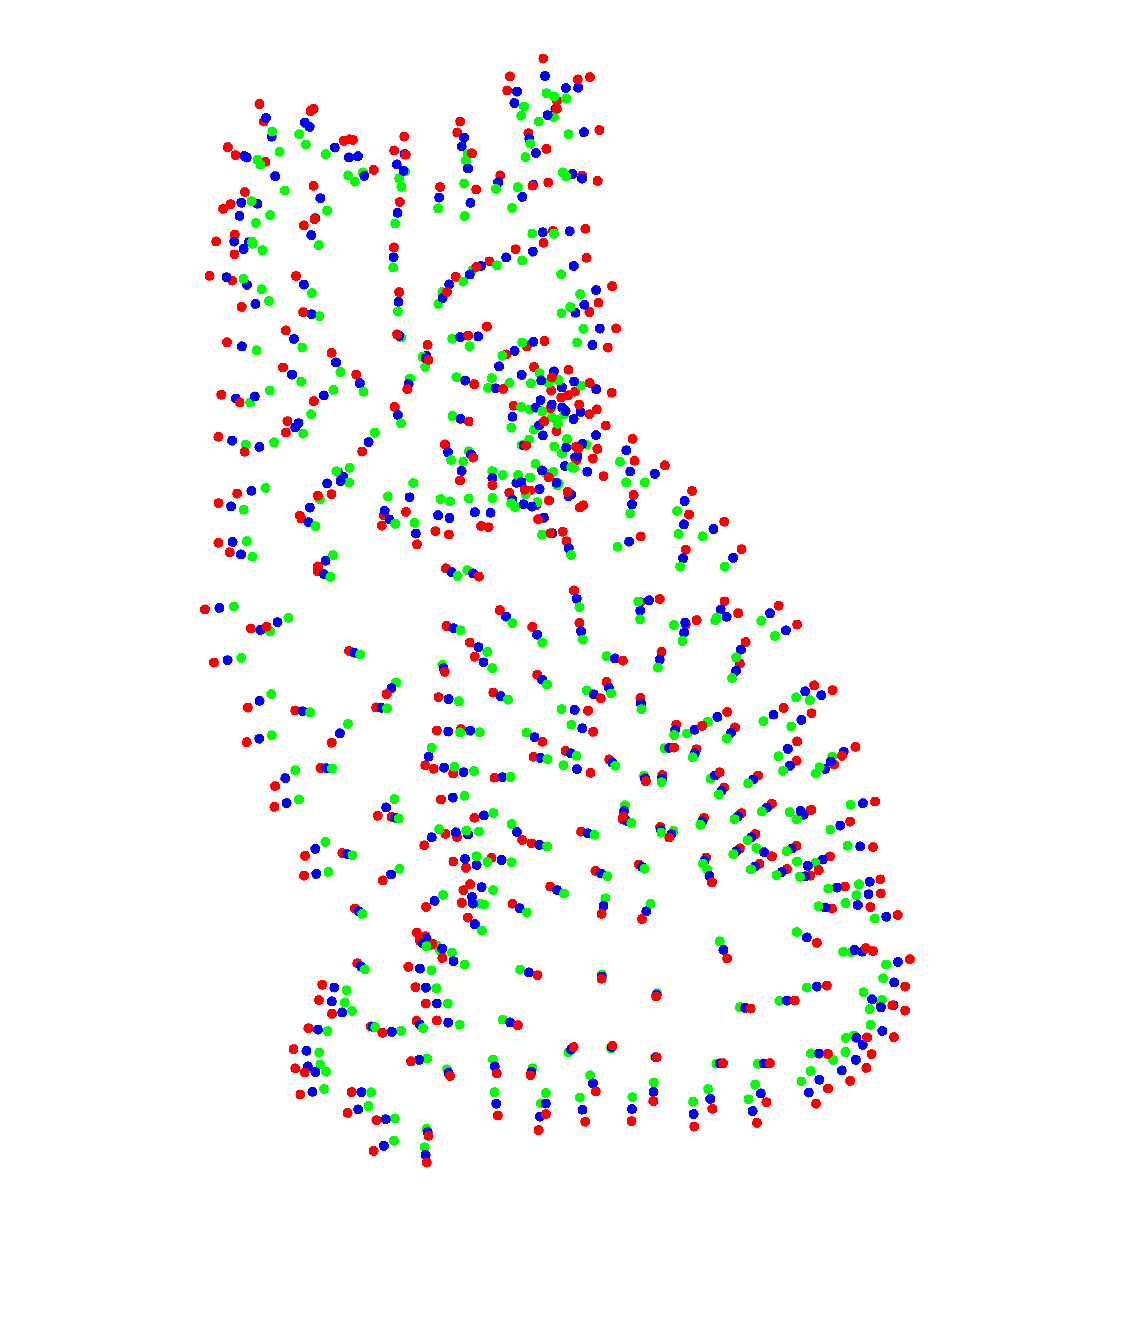
\includegraphics[width=0.4\linewidth]{cat_inoutpts.png}} % requires the graphicx package
   \caption{Input point cloud for the \emph{cat} mesh and inward/outward value constraints. In Fig.~\ref{fig:cat_inoutpts}, labels green, red and blue correspond to inside, outside and on the surface respectively. The blue points in Fig.~\ref{fig:cat_inoutpts} are the same as the black ones in Fig.~\ref{fig:cat_blackpts}.}
   \label{fig:cat_ptcloud}
\end{figure}

\subsection{Creating the constraints}
For this task, you need to complete the appropriate sections (keyboard callback,
keys '1' and '2') of \texttt{src/main.cpp}. Pressing key '1' displays the
input point cloud (this part has already been completed).
When key '2' is pressed, you must calculate and display the constraints
(points and implicit function values), storing them in
\texttt{constrained\_points},
\texttt{constrained\_values}. You should plot each constraint point in a color
chosen based on its type (inside/outside/surface) as in \pr{fig:cat_ptcloud}.

\emph{Relevant} \texttt{libigl} \emph{functions: } None.

\subsection{Implementing a spatial index to accelerate neighbor
calculations} To construct the MLS equations, you will perform queries
to find, for a query point $\vec q$:
\begin{itemize}
    \item the closest input point to $\vec q$ (needed while constructing
        inside/outside offset points); and
    \item all input points within distance $h$ of $\vec q$ (needed to
        select constraints with nonzero weight).
\end{itemize}
Although a simple loop over all points could answer these queries, it would be
slow for large point clouds. Improve the efficiency by implementing a simple
spatial index (a uniform grid at some resolution). By this, we mean binning
vertices into their enclosing grid cells and restricting the neighbor queries to
visit only the grid cells that could possibly satisfy the query. You can debug
this data structure by ensuring that it agrees with the brute-force for
loop implementation.

\emph{Relevant} \texttt{libigl} \emph{functions: } None.

\subsection*{Required output of \pr{sec:constraints}}
\begin{itemize}
\item{Visualization of the constrained points.}
\end{itemize}

\section{MLS Interpolation}
We now use MLS interpolation to construct an implicit function satisfying the
constraints as nearly as possible. We won't define the function with an explicit
formula; instead we characterize it as the linear combination of polynomial
basis functions that best satisfies the constraints in some sense. At a given
point $\x$, you evaluate this function by finding the ``optimal'' basis function
coefficients (which will vary from point to point!) and using these to combine
the basis function values at $\x$.

Complete the appropriate source code sections (inside the keyboard callback, key
'3') to evaluate the MLS function at every node of a regular volumetric
grid containing the point cloud. As an example, the provided code computes the
grid values for an implicit function representing a sphere (MLS wasn't used in
this case since the formula is known analytically). It corresponds to the point
cloud \texttt{sphere.off}. For a result using MLS see
Fig.~\ref{fig:cat_reconstr} (A).

\subsection{Create a grid sampling the 3D space}
Create a regular volumetric grid around your point cloud: compute the
axis-aligned bounding box of the point cloud, enlarge it slightly, and divide it
into uniform cells (cubes). The grid resolution is configured by
the global variable \texttt{resolution}, which can be changed in the GUI
sidebar. The marching cubes library needs to know the location of each grid
point, which you should store in the \texttt{grid\_points} array. The library
expects the points to be ordered lexicographically by their ($z$, $y$, $x$)
grid index; see the example grid construction provided in \texttt{createGrid}.

\emph{Relevant} \texttt{libigl} \emph{functions: } \texttt{igl::colon} can optionally be used to generate points.

\begin{figure}[h!]
   \centering
   \subfloat[Implicit function values at grid points]{
       \label{fig:cat_redgreenpts}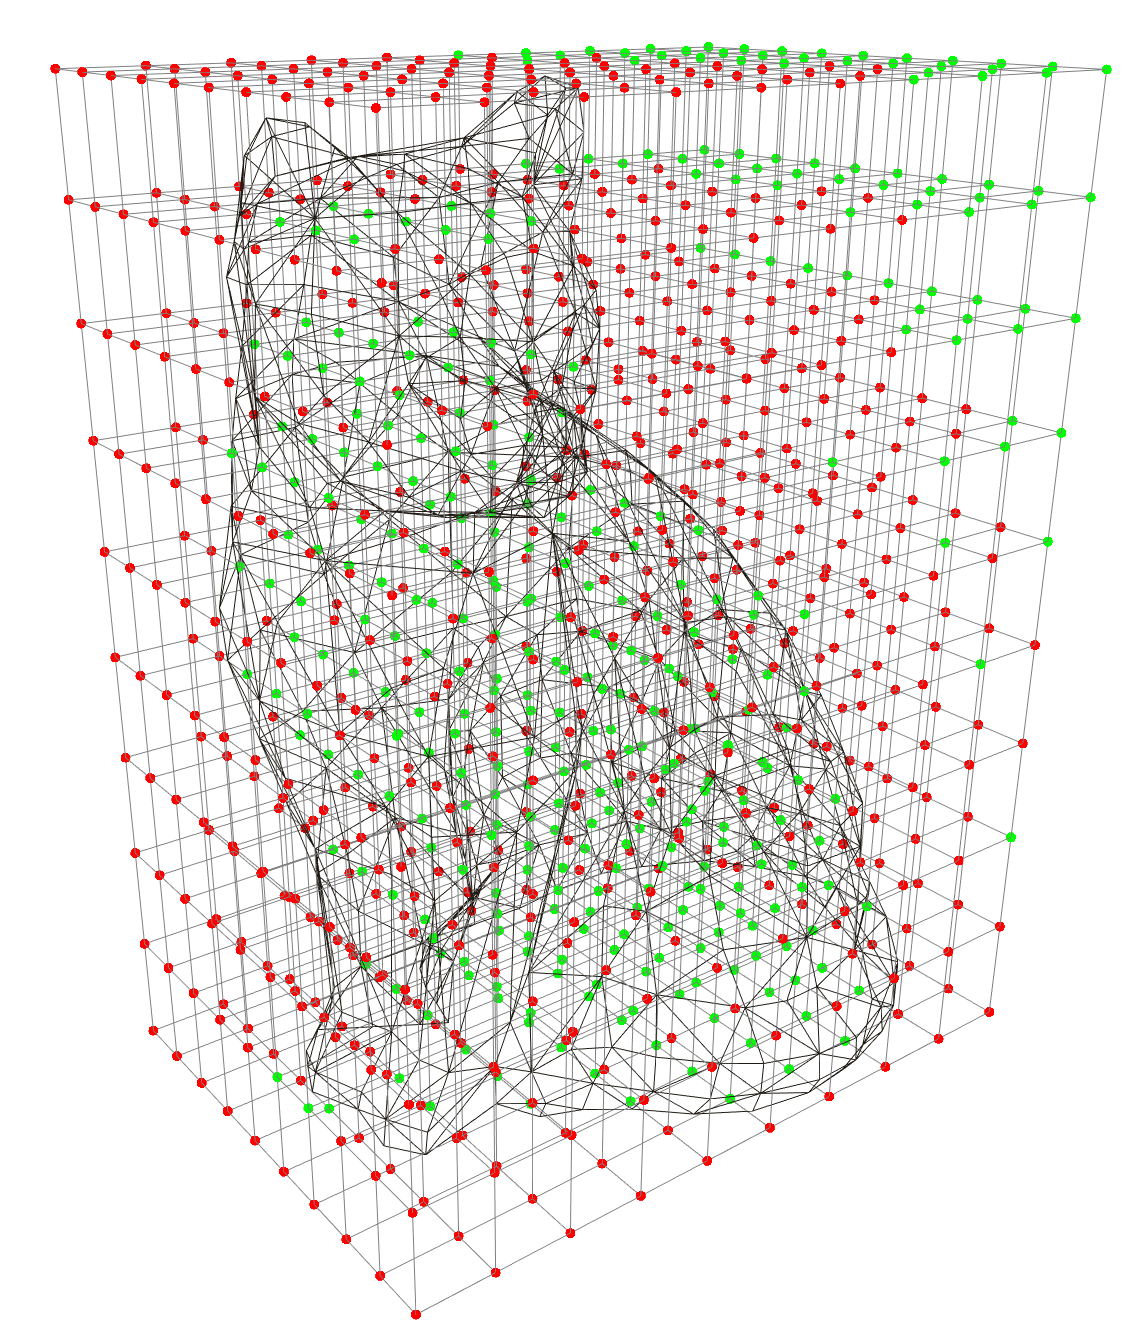
\includegraphics[width=0.4\linewidth]{cat_redgreen.png}
   }
\hspace{1cm}
   \subfloat[Marching Cubes result]{
       \label{fig:cat_final}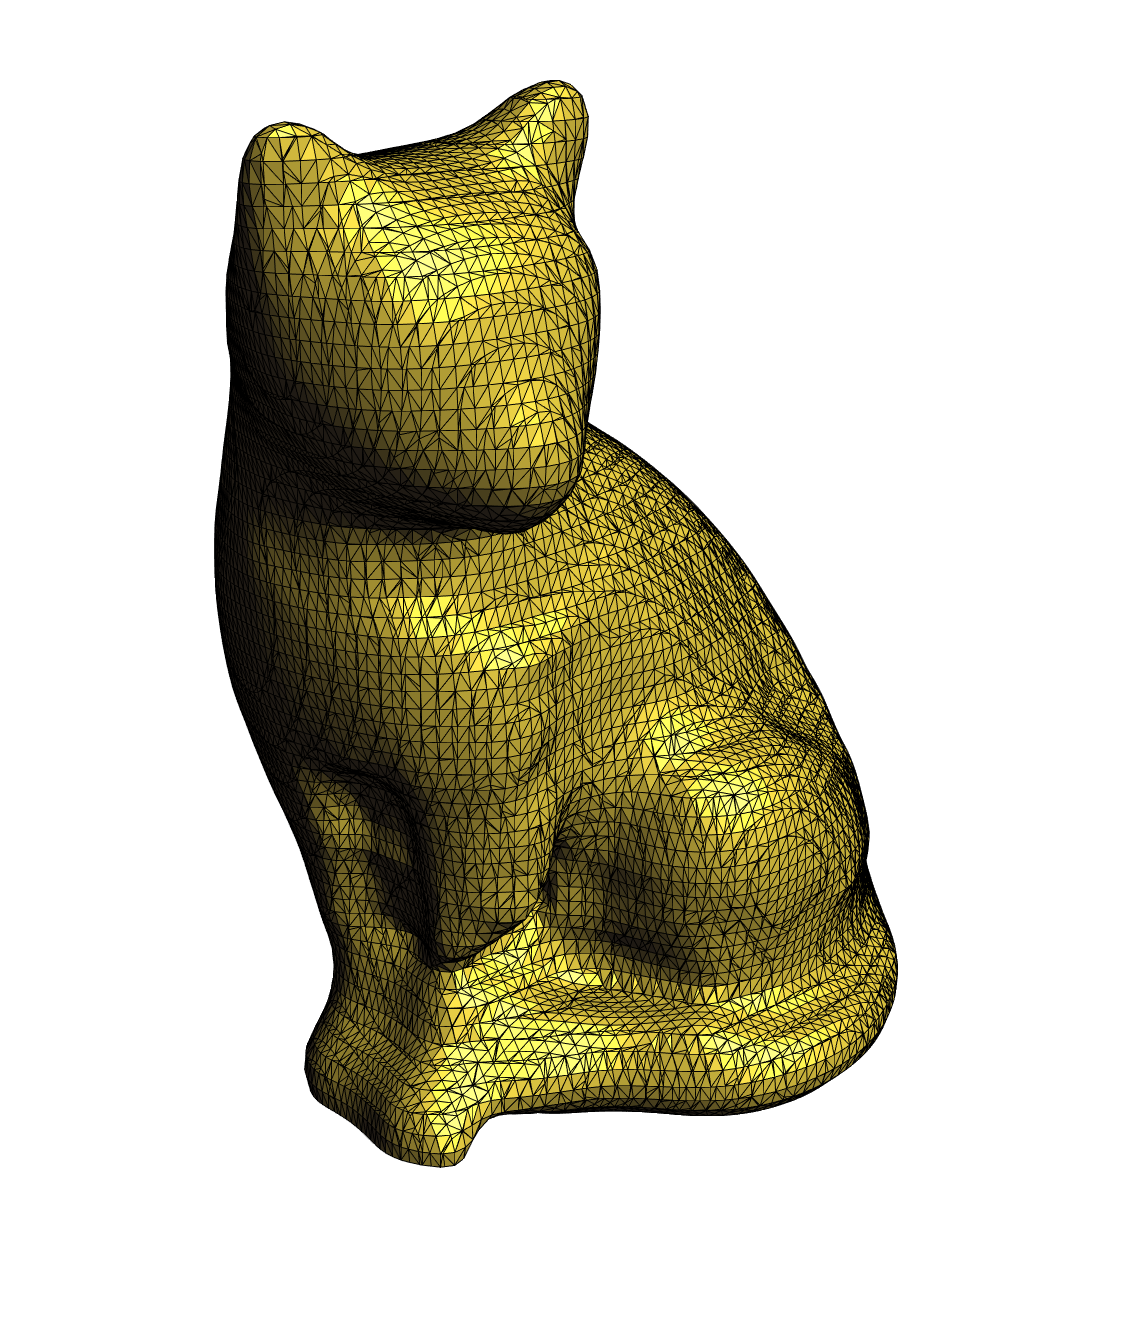
\includegraphics[width=0.4\linewidth]{cat_final.png}
   }
   \caption{MLS implicit function constructed from the value constraints shown
    in Fig.~\ref{fig:cat_ptcloud} and final reconstruction using marching cubes.
    In Fig.~\ref{fig:cat_redgreenpts}, green and red labels correspond to
    negative and positive values of the implicit function respectively.}
   \label{fig:cat_reconstr}
\end{figure}

\subsection{Evaluate the implicit function on the grid}
For each grid node of the grid, evaluate the implicit function $f(\x)$, whose
zero level set approximates the point cloud. Use the moving least squares
approximation presented in class and in the tutoring session. You should use the
Wendland weight function with radius configured by \texttt{wendlandRadius} and
degree $k = 0, 1, 2$ polynomial basis functions configured by
\texttt{polyDegree} (add these parameters to the GUI!). Only use the constraint
points with nonzero weight (which you can find efficiently using the spatial
index you created earlier). If no constraint points are within
\texttt{wendlandRadius} of the evaluation grid point, you can assign a large
positive (outside) value to the grid point.

Store the field value in the \texttt{grid\_values} array, using the same
ordering as in \texttt{grid\_points}. Render these values by coloring each grid
point red/green as already done for the sphere function (see
\pr{fig:cat_redgreenpts}). You can use the global variables
\texttt{grid\_colors} and \texttt{grid\_lines} to store the colors and the lines
of your grid. Code for displaying the grid is already provided (see function
\texttt{getLines} and the callback function).

\emph{Relevant} \texttt{libigl} \emph{functions: } \texttt{igl::slice} might
come in handy to extract the relevant constraint locations/values.

\subsection{Using a non-axis-aligned grid.}
The point cloud \texttt{luigi.off} is not aligned with the canonical axes.
Running reconstruction on an axis-aligned grid is wasteful in this case: many of
the grid points will lie far outside the object. Devise an automatic (and
general) way to align the grid to the data and implement it.

\vspace{1cm}
Required output of this section:
\begin{itemize}
\item{Screenshots of the grid with nodes colored according to their implicit function values.}
\end{itemize}

\section{Extracting the surface}

You can now use marching cubes to extract the zero isosurface from your grid.
The extraction has already been implemented and the surface is displayed when
key '4' is pressed. Add code to export your mesh in \text{off} format. For an
example result, see Fig.~\ref{fig:cat_reconstr} (B).

\emph{Relevant} \texttt{libigl} \emph{functions: } \texttt{igl::copyleft::marching\_cubes}, \texttt{igl::writeOFF}.

\vspace{1cm}
Required output of this section:
\begin{itemize}
\item{Screenshots of the reconstructed surfaces. Experiment with different
    parameter settings: grid resolution (also anisotropic in the 3 axes),
    Wendland function radius, polynomial degree. Add all these settings to the
        GUI to ease experimentation.}
\item{The reconstructed model in \texttt{off} format for every point-cloud
    dataset provided.}
\end{itemize}

\section*{Optional tasks}
\begin{enumerate}
\item \emph{(2 points)}
    Compute the closed-form gradient of the MLS approximation. Suggestion: A good
    strategy to solve this exercise is to write MLS explicitly in matrix
    form and then compute its gradient (a good reference for differentiating
    expressions with matrices can be found in ``\href{http://orion.uwaterloo.ca/~hwolkowi/matrixcookbook.pdf}{The Matrix Cookbook}'').

\item \emph{(2 points)}
    In ``\href{http://graphics.berkeley.edu/papers/Shen-IAI-2004-08/index.html}{Interpolating
    and Approximating Implicit Surfaces from Polygon Soup},'' normals are used
    differently to define the implicit surface. Instead of generating new
    sample points offset in the positive and negative normal directions, the
    paper uses the normal to define a linear function for
    each point cloud point: the signed distance to the tangent plane at the
    point. Then the values of these linear functions are interpolated by MLS.
    Implement Section 3.3 of the paper and append to your report a
    description of the method and how it compares to the original
    point-value-based approach.

%\item
%Assume that your input is a point cloud without normals. Estimate a normal for
    %every point and reconstruct the surface. Compare the results obtained with
    %the provided normals and the estimated normals on a single dataset.

\item
\emph{(1 point)}
        \href{http://www.cs.jhu.edu/~misha/MyPapers/ToG13.pdf}{Screened Poisson
        Surface Reconstruction} is a more modern technique that avoids some of
        the pitfalls of local reconstruction methods.

        An implementation is provided in \href{http://www.meshlab.net}{MeshLab}.
        A standalone implementation of this method is also provided by the
        authors
        \href{http://www.cs.jhu.edu/~misha/Code/PoissonRecon/Version9.01/}{here}
        with accompanying usage instructions and datasets. Compare your MLS
        reconstruction results to the surfaces obtained with this method, and
        try to understand the differences. Report your findings.

\end{enumerate}

% \bibliographystyle{plain}
% \bibliography{bib.bib}
\end{document}
